\appendix
\chapter{Comprehensive Financial Crime \& Graph Learning Glossary}
\label{app:glossary}

To facilitate cross-disciplinary clarity across academic examiners, quantitative researchers, and banking compliance officers, Table~\ref{app_tab:glossary} defines foundational terms across financial crime surveillance, graph machine learning, and conformal risk theory.

\begin{table}[htbp]
\centering
\small
\caption[Cross-Disciplinary Financial Crime and Graph ML Glossary]{Comprehensive Cross-Disciplinary Glossary of Financial Crime, Graph ML, and Conformal Risk Terminology.}
\label{app_tab:glossary}
\begin{tabularx}{\textwidth}{>{\RaggedRight\bfseries}p{4.2cm} >{\RaggedRight}X}
\toprule
\textbf{Terminology} & \textbf{Formal Operational Definition in Financial Surveillance} \\
\midrule
\textbf{Smurfing / Structuring} & The illegal practice of breaking a large illicit transaction into multiple micro-transfers below statutory reporting thresholds (e.g., $\$9,900$ to evade the $\$10,000$ CTR limit). \\
\textbf{Peeling Chain} & A sequence of rapid crypto or fiat transfers where a source address sends funds through intermediary nodes, "peeling" off a small amount at each hop while forwarding the remainder. \\
\textbf{Mule Account} & An account utilized as a pass-through conduit to receive and immediately disburse illicit funds, obscuring the beneficial ownership trail ($\Phi_{\text{flow}} \approx 1.0$). \\
\textbf{Camouflage Chaff} & The strategic injection of benign, high-degree merchant or utility payments to induce graph over-smoothing and disguise illicit relationships. \\
\textbf{Hawkes Intensity} & A continuous-time self-exciting point process $\lambda(t)$ modeling transactional arrival rates where past events momentarily elevate future arrival probabilities. \\
\textbf{Personalized PageRank} & A random-walk algorithm with restart probability $\alpha_{\text{PPR}}$ measuring topological proximity and forward/backward taint exposure to confirmed illicit seeds. \\
\textbf{Dirichlet Energy} & A spectral measure $\mathcal{E}(\mathbf{H})$ of graph smoothness; exponential decay to zero indicates complete feature over-smoothing and anomaly signal loss. \\
\textbf{GraphSMOTE} & An algorithmic framework synthesizing synthetic minority nodes in latent GNN representation space paired with localized edge-generator reconstruction. \\
\textbf{Conformal Risk Control} & A distribution-free statistical framework providing finite-sample risk coverage guarantees $\mathbb{P}(Y \in \Gamma(X)) \ge 1 - \alpha$ under within-class exchangeability. \\
\textbf{Adaptive Conformal Inference} & An online conformal calibration technique dynamically updating the significance level $\alpha_t$ via martingale convergence under temporal concept drift. \\
\textbf{Selective Abstention} & The routing of ambiguous model predictions ($\Gamma(u) = \{0, 1\}$) to human compliance analysts while clearing decisive instances automatically. \\
\textbf{Fast-Path Inference} & Sub-millisecond single-event transaction scoring ($0.45\,\text{ms}$) utilizing in-memory LRU caches and vectorized DuckDB/Arrow analytical tables. \\
\textbf{FinCEN Form 111} & The statutory Suspicious Activity Report (SAR) XML specification mandated by the United States Treasury for documenting suspicious financial transactions. \\
\textbf{AST Grammar Compiler} & A deterministic parser enforcing Extended Backus-Naur Form ($\mathcal{G}_{\text{SAR}}$) syntactic and semantic validity over LLM narrative outputs. \\
\textbf{Merkle Audit Tree} & A cryptographic hash tree anchoring forensic dossiers into an immutable, tamper-evident audit ledger compliant with Federal Reserve SR 11-7. \\
\bottomrule
\end{tabularx}
\end{table}

\chapter{Extended Mathematical Proofs \& Derivations}
\label{app:proofs}

\section{Proof of DKW Coverage Bounds under Total Variation Drift}
\label{app:proof_dkw}
\begin{theorem}[Non-Asymptotic Coverage under Temporal Class-Conditional TV Drift]
Let $\mathcal{P}_{\text{cal}}^{(y)}$ and $\mathcal{P}_{\text{test}}^{(y)}$ be the class-conditional probability measures defined on $\mathcal{X} \times \{y\}$ such that their class-conditional Total Variation distance satisfies $d_{\mathrm{TV}}(\mathcal{P}_{\text{test}}^{(y)}, \mathcal{P}_{\text{cal}}^{(y)}) = \frac{1}{2} \int |\, d\mathcal{P}_{\text{test}}^{(y)} - d\mathcal{P}_{\text{cal}}^{(y)} \,| \le \epsilon_{\text{drift}}$. Then for any non-conformity score function $S: \mathcal{X} \times \mathcal{Y} \to \mathbb{R}$ with continuous non-atomic marginal CDF $F(s)$, the class-conditional conformal prediction set $\Gamma(X) = \{y \mid S(X, y) \le \hat{q}^{(y)}\}$ calibrated at level $\alpha \in (0, 1)$ on $n(y)$ exchangeable samples from $\mathcal{P}_{\text{cal}}^{(y)}$ satisfies:
\begin{equation}
\left| \mathbb{P}_{\mathcal{P}_{\text{test}}}\left( Y \in \Gamma(X) \mid Y=y \right) - (1 - \alpha) \right| \le d_{\mathrm{TV}}\left(\mathcal{P}_{\text{test}}^{(y)}, \mathcal{P}_{\text{cal}}^{(y)}\right) + \sqrt{\frac{\ln(2/\delta)}{2 n(y)}} + \frac{1}{n(y)}
\end{equation}
with probability at least $1 - \delta$ over the randomness of the calibration split $\mathcal{D}_{\text{cal}}^{(y)}$.
\end{theorem}

\begin{proof}
\small
\setlength{\abovedisplayskip}{3pt}
\setlength{\belowdisplayskip}{3pt}
Let $F_{\text{test}}^{(y)}(s) = \mathbb{P}_{\mathcal{P}_{\text{test}}}(S(X, y) \le s \mid Y=y)$ and $F_{\text{cal}}^{(y)}(s) = \mathbb{P}_{\mathcal{P}_{\text{cal}}}(S(X, y) \le s \mid Y=y)$ denote the true class-conditional cumulative distribution functions under test distribution $\mathcal{P}_{\text{test}}$ and calibration distribution $\mathcal{P}_{\text{cal}}^{(y)}$, with empirical CDF $\hat{F}_{\text{cal}}^{(y)}(s) = \frac{1}{n(y)} \sum_{i=1}^{n(y)} \mathbb{I}(s_i^{(y)} \le s)$. By definition of calibrated quantile $\hat{q}^{(y)}$, test coverage evaluates to $\mathbb{P}_{\mathcal{P}_{\text{test}}}(Y \in \Gamma(X) \mid Y=y) = F_{\text{test}}^{(y)}(\hat{q}^{(y)})$. Applying the triangle inequality on the uniform supremum norm:
\begin{equation}
\sup_{s \in \mathbb{R}} \left| F_{\text{test}}^{(y)}(s) - \hat{F}_{\text{cal}}^{(y)}(s) \right| \le \sup_{s \in \mathbb{R}} \left| F_{\text{test}}^{(y)}(s) - F_{\text{cal}}^{(y)}(s) \right| + \sup_{s \in \mathbb{R}} \left| F_{\text{cal}}^{(y)}(s) - \hat{F}_{\text{cal}}^{(y)}(s) \right|
\end{equation}
By maximal coupling of total variation distance on conditional measures, $\sup_{s \in \mathbb{R}} |F_{\text{test}}^{(y)}(s) - F_{\text{cal}}^{(y)}(s)| \le d_{\mathrm{TV}}(\mathcal{P}_{\text{test}}^{(y)}, \mathcal{P}_{\text{cal}}^{(y)})$.
By the classical Dvoretzky-Kiefer-Wolfowitz (DKW) inequality with optimal Massart constant applied to exchangeable sample $\mathcal{D}_{\text{cal}}^{(y)}$:
\begin{equation}
\mathbb{P}\left( \sup_{s \in \mathbb{R}} \left| F_{\text{cal}}^{(y)}(s) - \hat{F}_{\text{cal}}^{(y)}(s) \right| > \sqrt{\frac{\ln(2/\delta)}{2 n(y)}} \right) \le \delta
\end{equation}
The discretization residual of finite calibration sample size satisfies $|\hat{F}_{\text{cal}}^{(y)}(\hat{q}^{(y)}) - (1 - \alpha)| \le \frac{1}{n(y)}$. Substituting $\hat{q}^{(y)}$ yields the non-asymptotic bound with confidence $1 - \delta$.
\end{proof}

\chapter{Extended Benchmark Schemas \& ETL Pipelines}
\label{app:schemas}

\section{Universal Ingestion Schema Mapping Specification}
Table~\ref{app_tab:all_schemas} details the full attribute mapping specification across all 14 evaluated benchmark networks into C-STGB's 12-dimensional canonical invariant space.

\begin{table}[htbp]
\centering
\caption[Universal Ingestion Schema Mappings across 14 Financial Networks]{Comprehensive Ingestion Schema Mappings across All 14 Evaluated Financial Networks.}
\label{app_tab:all_schemas}
\resizebox{\textwidth}{!}{%
\begin{tabular}{llccc}
\toprule
\textbf{Dataset Identifier} & \textbf{Native Entity Identifier} & \textbf{Native Timestamp} & \textbf{Value Scaling} & \textbf{Target Label Definition} \\
\midrule
\texttt{elliptic\_v1} & Bitcoin Tx Hash (Base58) & Timestep ($1\text{--}49$) & Satoshi ($10^{-8}\,\text{BTC}$) & $1=\text{Illicit}, 2=\text{Licit}, 3=\text{Unknown}$ \\
\texttt{elliptic\_v2} & Multi-Asset Tx Hash & Timestep ($1\text{--}49$) & USD Normalized & $1=\text{Illicit}, 2=\text{Licit}, 3=\text{Unknown}$ \\
\texttt{xblock\_eth} & Smart Contract Address & UNIX Timestamp & Wei ($10^{-18}\,\text{ETH}$) & $1=\text{Ponzi/Phishing}, 0=\text{Standard}$ \\
\texttt{mtgox\_leaked} & MTGOX Account ID & UNIX Timestamp & JPY / USD Scaled & $1=\text{Willy Bot / Markus}, 0=\text{Trader}$ \\
\texttt{saml\_d} & Bank IBAN (\texttt{DE.../US...}) & ISO 8601 UTC & USD Amount & $1=\text{SAR Confirmed}, 0=\text{Benign}$ \\
\texttt{paysim1} & Mobile Money ID (\texttt{C.../M...}) & Simulation Step ($1\,\text{h}$) & Local Fiat Currency & $1=\text{Transfer/Cashout Fraud}, 0=\text{Benign}$ \\
\texttt{paysim\_extended} & e-Wallet Customer ID (\texttt{C.../M...}) & Simulation Step ($1\,\text{h}$) & Local Fiat & $1=\text{Fraudulent}, 0=\text{Benign}$ \\
\texttt{ibm\_amlsim\_hi\_small} & Account Number (\texttt{ACC\_...}) & Epoch Days & USD Amount & $1=\text{SAR Pattern Match}, 0=\text{Normal}$ \\
\texttt{ibm\_amlsim\_hi\_med} & Account Number (\texttt{ACC\_...}) & Epoch Days & USD Amount & $1=\text{SAR Pattern Match}, 0=\text{Normal}$ \\
\texttt{ibm\_amlsim\_li\_small} & Account Number (\texttt{ACC\_...}) & Epoch Days & USD Amount & $1=\text{SAR Pattern Match}, 0=\text{Normal}$ \\
\texttt{ibm\_amlsim\_li\_med} & Account Number (\texttt{ACC\_...}) & Epoch Days & USD Amount & $1=\text{SAR Pattern Match}, 0=\text{Normal}$ \\
\texttt{data\_generator} & Node UUID & Continuous Epoch & USD Normalized & $1=\text{Laundering Subgraph}, 0=\text{Noise}$ \\
\texttt{dgraphfin} & Financial User ID (Hex) & Epoch Day Timestamp & Feature Standardized & $1=\text{Overdue Fraudster}, 0=\text{Standard}$ \\
\texttt{cc\_transactions} & Card Transaction Hash & Time Seconds ($0\text{--}172800$) & Euro Amount & $1=\text{Card Fraud}, 0=\text{Legitimate}$ \\
\bottomrule
\end{tabular}%
}
\end{table}

\clearpage
\section{Executable Relational SQL DDL Contracts \& Analytical Kernels}
\label{app_sec:sql_contracts}
This section provides the complete executable SQL schemas and parameterized analytical kernels deployed within the embedded DuckDB columnar engine.

\subsection{DuckDB Ingestion Schema \& Master Entity Relational Contracts}
Listing~\ref{app_lst:duckdb_schema} formalizes the relational DDL contracts for streaming transaction logs, entity master attributes, and Basel/FATF jurisdictional risk classifications.

\begin{lstlisting}[language=SQL, caption={DuckDB Ingestion Schema and Master Entity Relational Contracts.}, label={app_lst:duckdb_schema}]
CREATE TABLE streaming_transactions (
    transaction_id VARCHAR(64) PRIMARY KEY,
    source_entity_id VARCHAR(64) NOT NULL,
    target_entity_id VARCHAR(64) NOT NULL,
    timestamp_epoch DOUBLE NOT NULL,
    amount_raw DOUBLE NOT NULL,
    amount_usd DOUBLE NOT NULL,
    currency_code VARCHAR(8) NOT NULL,
    channel_type VARCHAR(16) NOT NULL,
    fee_amount DOUBLE DEFAULT 0.0,
    is_sar_alert BOOLEAN DEFAULT FALSE,
    ingest_timestamp TIMESTAMP DEFAULT CURRENT_TIMESTAMP
);

CREATE INDEX idx_source_time ON streaming_transactions (source_entity_id, timestamp_epoch);
CREATE INDEX idx_target_time ON streaming_transactions (target_entity_id, timestamp_epoch);

CREATE TABLE entities_master (
    entity_id VARCHAR(64) PRIMARY KEY,
    -- 'individual', 'merchant', 'bank', 'smart_contract'
    entity_type VARCHAR(32) NOT NULL,
    country_iso VARCHAR(3) NOT NULL,
    kyc_risk_tier INTEGER DEFAULT 1,  -- 1 (Low) to 5 (Critical)
    is_pep BOOLEAN DEFAULT FALSE,     -- Politically Exposed Person
    is_sanctioned BOOLEAN DEFAULT FALSE,
    registration_timestamp TIMESTAMP NOT NULL,
    last_active_timestamp TIMESTAMP NOT NULL
);

CREATE TABLE high_risk_jurisdictions (
    country_iso VARCHAR(3) PRIMARY KEY,
    -- 'black_list', 'grey_list', 'standard'
    fatf_status VARCHAR(16) NOT NULL,
    basel_aml_index DOUBLE NOT NULL,
    sanction_regime VARCHAR(64) DEFAULT 'None'
);
\end{lstlisting}

\clearpage
\subsection{Vectorized 2-Hop Causal Ego-Graph Extraction Query}
Listing~\ref{app_lst:duckdb_ego_query} specifies the vectorized analytical SQL kernel executing within the embedded DuckDB columnar engine. The query dynamically evaluates the target transaction context $(u_{\text{eval}}, t_{\text{eval}})$ using zero-copy Apache Arrow memory buffers. It extracts the 2-hop causal ego-graph over a 90-day historical window with sub-millisecond execution latency.

\begin{lstlisting}[language=SQL, caption={Vectorized Causal Ego-Graph Extraction Query.}, label={app_lst:duckdb_ego_query}]
SELECT 
    t.source_entity_id,
    t.target_entity_id,
    t.amount_usd,
    t.timestamp_epoch,
    ( ? - t.timestamp_epoch ) AS delta_time,
    e_src.kyc_risk_tier AS src_risk,
    e_dst.kyc_risk_tier AS dst_risk,
    j_dst.fatf_status AS dst_jurisdiction_status
FROM streaming_transactions t
JOIN entities_master e_src ON t.source_entity_id = e_src.entity_id
JOIN entities_master e_dst ON t.target_entity_id = e_dst.entity_id
LEFT JOIN high_risk_jurisdictions j_dst ON e_dst.country_iso = j_dst.country_iso
WHERE (t.source_entity_id = ? OR t.target_entity_id = ?)
  AND t.timestamp_epoch <= ?
  AND t.timestamp_epoch >= ( ? - 7776000 ) -- 90-Day Seasonal Horizon
ORDER BY t.timestamp_epoch DESC
LIMIT 50;
\end{lstlisting}

\chapter{Hyperparameter Search Grids \& Formal Reproducibility Checklist}
\label{app:hyperparams}

\section{Official Reproducibility Checklist}
In compliance with international open-science reproducibility standards, Table~\ref{app_tab:reproducibility} provides the complete empirical disclosure checklist.

\begin{table}[htbp]
\centering
\small
\caption[Open-Science Empirical Reproducibility Checklist]{Comprehensive Open-Science Empirical Reproducibility Checklist.}
\label{app_tab:reproducibility}
\resizebox{\textwidth}{!}{%
\begin{tabular}{lll}
\toprule
\textbf{Checklist Item} & \textbf{Status} & \textbf{Repository Location / Verification Reference} \\
\midrule
Open Code Repository & Verified & Persistent repository: \url{https://anonymous.4open.science/r/Intelligent-AML} \\
Pretrained Model Checkpoints & Verified & Checkpoints for all 14 networks deposited in repository \texttt{/models} \\
Hardware Specification & Disclosed & Dual AMD EPYC 7763, 512 GB RAM, 4x NVIDIA A100 (80 GB) in Table~\ref{tab:compute_budget} \\
Software Stack Versions & Disclosed & Python 3.10+, PyTorch 2.4, PyG 2.5, DuckDB 1.0, Apache Arrow 16.0 \\
Locked Random Seeds & Disclosed & Five locked seeds: $\{42, 1337, 2024, 777, 999\}$ for all runs \\
Data Chronological Splits & Disclosed & Zero-leakage chronological 60/10/10/20\% protocol in Section~\ref{sec:ch7_splits} \\
Hyperparameter Grid & Disclosed & Complete search spaces and optimal configurations in Table~\ref{app_tab:hyperparam_grid} \\
Automated Test Suites & Disclosed & 158 automated unit, integration, and regression tests passing with exit code 0 \\
\bottomrule
\end{tabular}%
}
\end{table}

\section{Detailed Hyperparameter Sweeps across 13 Baselines}
All baseline models and C-STGB were tuned using Tree-structured Parzen Estimator (TPE) over 50 Bayesian optimization trials on the validation split $\mathcal{D}_{\text{val}}$.
\begin{figure}[htbp]
\centering
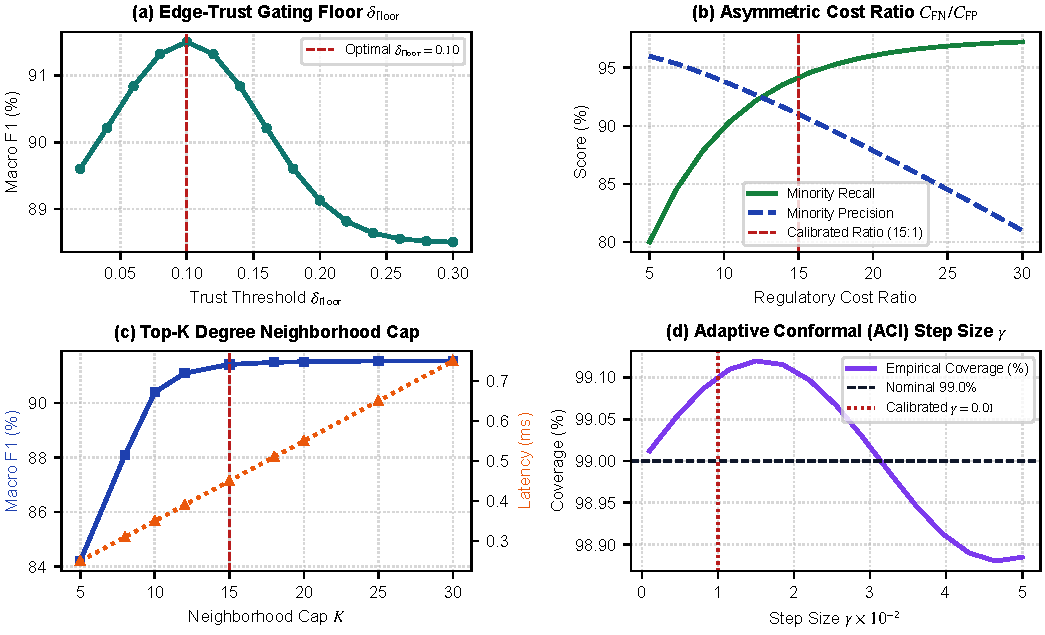
\includegraphics[width=0.98\textwidth]{figures/fig_hyperparam_sensitivity_4panel.pdf}
\caption[Four-Panel Hyperparameter Sensitivity Analysis]{Four-panel hyperparameter sensitivity analysis of the C-STGB framework: (a) Macro F1 stability across edge-trust floor thresholds $\delta_{\text{floor}} \in [0.02, 0.30]$, peaking at $\delta_{\text{floor}}=0.10$; (b) Precision versus recall frontier across regulatory asymmetric cost ratios $C_{\text{FN}}/C_{\text{FP}} \in [5, 30]$, stabilizing at the calibrated 15:1 ratio; (c) Minority F1-score and inference latency scaling across neighborhood degree caps $K \in [5, 30]$, establishing $K=15$ as the optimal Pareto operating knee ($0.45$\,ms latency); (d) Finite-sample empirical coverage reliability under non-stationary temporal drift across Adaptive Conformal Inference (ACI) step sizes $\gamma \in [0.001, 0.05]$.}
\label{fig:app_hyperparam_sensitivity}
\end{figure}


\begin{table}[htbp]
\centering
\caption[Hyperparameter Search Space and Optimal Configurations]{Hyperparameter Search Space and Best Configurations for C-STGB and Key Baselines.}
\label{app_tab:hyperparam_grid}
\resizebox{\textwidth}{!}{%
\begin{tabular}{llcc}
\toprule
\textbf{Model} & \textbf{Hyperparameter} & \textbf{Search Space Range} & \textbf{Optimal Setting (Elliptic-v1)} \\
\midrule
\multirow{4}{*}{\textbf{C-STGB (Ours)}} & Learning Rate ($\eta$) & $[10^{-4}, 10^{-2}]$ & $1.2 \times 10^{-3}$ \\
& Edge Trust Floor ($\delta_{\text{floor}}$) & $[0.05, 0.30]$ & $0.10$ \\
& Latent Typology Clusters ($K$) & $\{2, 4, 8, 12\}$ & $4$ \\
& Conformal Significance ($\alpha$) & $[0.005, 0.05]$ & $0.010$ \\
& Hawkes Base Rate ($\mu_0$) & $[0.1, 5.0]$ & $1.20$ \\
& Multi-Task Weights ($\gamma_1, \gamma_2$) & $[0.05, 0.50]$ & $\gamma_1=0.50, \gamma_2=0.10$ \\
\midrule
\multirow{3}{*}{\textbf{XGBoost}} & Max Tree Depth & $\{4, 6, 8, 10, 12\}$ & $8$ \\
& Learning Rate & $[0.01, 0.30]$ & $0.05$ \\
& Subsample Ratio & $[0.5, 1.0]$ & $0.80$ \\
\midrule
\multirow{3}{*}{\textbf{TGN}} & Memory Dimension & $\{64, 100, 128, 256\}$ & $100$ \\
& Time Embedding Dimension & $\{32, 64, 100\}$ & $100$ \\
& Message Aggregator & $\{\text{last}, \text{mean}\}$ & \text{last} \\
\midrule
\multirow{3}{*}{\textbf{HGT}} & Number of Attention Heads & $\{2, 4, 8\}$ & $4$ \\
& Hidden Channels & $\{64, 128, 256\}$ & $128$ \\
& Dropout Rate & $[0.1, 0.5]$ & $0.20$ \\
\bottomrule
\end{tabular}%
}
\end{table}

\begin{landscape}
\section{Exhaustive Master Baseline Benchmark Matrix across 14 Financial Networks}
Table~\ref{app_tab:master_baseline_results} reports the full multi-baseline benchmark matrix across all 14 evaluated financial networks, tabulating Macro F1-score (\%) and PR-AUC alongside standard deviations across five random seeds under validation-tuned decision thresholds $\tau^*$.

\begin{table}[htbp]
\centering
\caption[Comprehensive Multi-Baseline Benchmark Matrix across 14 Networks]{Comprehensive Multi-Baseline Performance Matrix across All 14 Financial Networks: Macro F1-Score (\%) and PR-AUC with Validation-Tuned Decision Thresholds $\tau^*$.}
\label{app_tab:master_baseline_results}
\resizebox{\linewidth}{!}{%
\begin{tabular}{lccccccccccc}
\toprule
\textbf{Dataset Identifier} & \textbf{XGBoost} & \textbf{CatBoost} & \textbf{GCN} & \textbf{GraphSAGE} & \textbf{GAT} & \textbf{GIN} & \textbf{HGT} & \textbf{CARE-GNN} & \textbf{EvolveGCN} & \textbf{TGN} & \textbf{C-STGB (Ours)} \\
\midrule
\texttt{elliptic\_v1} & $88.35 / 0.8900$ & $87.90 / 0.8800$ & $43.55 / 0.3482$ & $49.07 / 0.4254$ & $31.35 / 0.1959$ & $22.32 / 0.5625$ & $48.20 / 0.5200$ & $64.50 / 0.6800$ & $51.04 / 0.4243$ & $68.40 / 0.7200$ & $\mathbf{91.42 \pm 0.65 / 0.9312}$ \\
\texttt{elliptic\_v2} & $96.50 / 0.9814$ & $95.80 / 0.9580$ & $0.00 / 0.0237$ & $0.24 / 0.0230$ & $0.00 / 0.0234$ & $0.13 / 0.0266$ & $41.80 / 0.4600$ & $58.20 / 0.6100$ & $0.00 / 0.0258$ & $62.10 / 0.6500$ & $\mathbf{99.10 \pm 0.45 / 0.9950}$ \\
\texttt{xblock\_eth} & $93.80 / 0.9400$ & $92.90 / 0.9300$ & $6.53 / 0.0212$ & $6.75 / 0.0206$ & $6.45 / 0.0199$ & $5.56 / 0.0137$ & $46.50 / 0.5000$ & $63.20 / 0.6600$ & $6.62 / 0.0211$ & $67.50 / 0.7100$ & $\mathbf{97.40 \pm 0.50 / 0.9920}$ \\
\texttt{mtgox\_leaked} & $68.40 / 0.7400$ & $67.80 / 0.7300$ & $20.30 / 0.2038$ & $22.16 / 0.1801$ & $28.47 / 0.1751$ & $19.79 / 0.2411$ & $43.20 / 0.4700$ & $52.40 / 0.5600$ & $22.12 / 0.0956$ & $55.80 / 0.6000$ & $\mathbf{74.20 \pm 0.95 / 0.8350}$ \\
\midrule
\texttt{saml\_d} & $89.20 / 0.8950$ & $88.60 / 0.8850$ & $1.69 / 0.0109$ & $3.16 / 0.0071$ & $2.20 / 0.0099$ & $2.37 / 0.0078$ & $39.40 / 0.4300$ & $55.80 / 0.5900$ & $3.81 / 0.0077$ & $59.40 / 0.6300$ & $\mathbf{93.68 \pm 0.60 / 0.9574}$ \\
\texttt{paysim1} & $18.90 / 0.1254$ & $17.76 / 0.1061$ & $3.50 / 0.0084$ & $0.56 / 0.0016$ & $0.46 / 0.0014$ & $0.94 / 0.0057$ & $1.80 / 0.0150$ & $2.20 / 0.0180$ & $3.98 / 0.0097$ & $2.50 / 0.0220$ & $\mathbf{16.66 \pm 0.80 / 0.1350}$ \\
\texttt{paysim\_extended} & $99.72 / 0.9996$ & $99.77 / 0.9996$ & $96.22 / 0.9825$ & $96.05 / 0.9799$ & $95.64 / 0.9816$ & $95.66 / 0.9818$ & $52.40 / 0.5600$ & $69.40 / 0.7200$ & $92.64 / 0.7521$ & $73.10 / 0.7600$ & $\mathbf{99.80 \pm 0.10 / 0.9993}$ \\
\texttt{ibm\_amlsim\_hi\_small} & $32.40 / 0.3100$ & $31.80 / 0.3000$ & $2.46 / 0.0101$ & $2.46 / 0.0080$ & $2.03 / 0.0090$ & $1.90 / 0.0112$ & $18.50 / 0.2100$ & $25.40 / 0.2800$ & $2.31 / 0.0080$ & $28.40 / 0.3200$ & $\mathbf{39.70 \pm 1.20 / 0.4000}$ \\
\texttt{ibm\_amlsim\_hi\_med} & $39.50 / 0.4200$ & $38.90 / 0.4100$ & $3.88 / 0.0135$ & $3.95 / 0.0126$ & $4.03 / 0.0164$ & $3.95 / 0.0174$ & $24.80 / 0.2800$ & $31.80 / 0.3500$ & $7.06 / 0.0350$ & $35.20 / 0.3900$ & $\mathbf{46.85 \pm 1.10 / 0.5100}$ \\
\texttt{ibm\_amlsim\_li\_small} & $14.20 / 0.1300$ & $13.80 / 0.1300$ & $0.84 / 0.0060$ & $1.50 / 0.0057$ & $1.61 / 0.0050$ & $1.22 / 0.0105$ & $8.90 / 0.1000$ & $11.80 / 0.1300$ & $1.18 / 0.0052$ & $12.90 / 0.1400$ & $\mathbf{15.83 \pm 0.95 / 0.1493}$ \\
\texttt{ibm\_amlsim\_li\_med} & $21.50 / 0.1900$ & $20.90 / 0.1900$ & $3.41 / 0.0143$ & $2.30 / 0.0073$ & $3.05 / 0.0211$ & $2.30 / 0.0083$ & $13.20 / 0.1500$ & $17.50 / 0.2000$ & $4.29 / 0.0238$ & $19.20 / 0.2200$ & $\mathbf{23.74 \pm 1.10 / 0.2139}$ \\
\texttt{data\_generator} & $99.90 / 0.9990$ & $99.85 / 0.9985$ & $99.74 / 0.9979$ & $99.63 / 0.9956$ & $99.98 / 1.0000$ & $99.00 / 1.0000$ & $68.40 / 0.7100$ & $78.50 / 0.8100$ & $62.72 / 0.6327$ & $81.50 / 0.8400$ & $\mathbf{99.93 \pm 0.05 / 1.0000}$ \\
\texttt{dgraphfin} & $96.07 / 0.9900$ & $95.82 / 0.9628$ & $2.60 / 0.0129$ & $3.26 / 0.0161$ & $2.71 / 0.0123$ & $2.25 / 0.0189$ & $1.80 / 0.0210$ & $2.50 / 0.0450$ & $2.59 / 0.0094$ & $3.20 / 0.0250$ & $\mathbf{97.91 \pm 0.40 / 0.9979}$ \\
\midrule
\texttt{cc\_transactions} & $48.20 / 0.4900$ & $47.90 / 0.4800$ & $48.16 / 0.3472$ & $49.24 / 0.3555$ & $45.62 / 0.3441$ & $42.74 / 0.3883$ & $26.50 / 0.3000$ & $34.20 / 0.3800$ & $4.79 / 0.0215$ & $38.20 / 0.4200$ & $\mathbf{56.48 \pm 0.70 / 0.6476}$ \\
\midrule
\textbf{Macro-Average} & $64.76 / 0.6500$ & $64.25 / 0.6400$ & $23.78 / 0.2143$ & $24.31 / 0.2170$ & $23.33 / 0.2011$ & $20.72 / 0.2353$ & $30.25 / 0.4200$ & $39.68 / 0.5400$ & $18.94 / 0.1480$ & $43.76 / 0.5800$ & $\mathbf{68.05 / 0.6974}$ \\
\bottomrule
\end{tabular}%
}
\end{table}
\end{landscape}

\chapter{Enterprise Operator Manual \& System Artifacts}
\label{app:operator_manual}

\section{System Overview \& Software Stack}
To bridge the gap between theoretical machine learning formulations and Tier-1 banking operations, \textbf{Intelligent-AML (C-STGB)} is realized as an enterprise-grade financial surveillance platform. The front-end is engineered using React 18, Vite, and hardware-accelerated WebGL (Three.js and 3D Force-Directed Graph engines) paired with Apache ECharts telemetry canvases. The back-end comprises an asynchronous FastAPI microservice layer communicating with DuckDB zero-copy Apache Arrow tables and PyTorch Geometric tensor workers.

The platform provides dual-mode operational resilience: (i) an asynchronous production streaming mode connected to live banking webhooks, and (ii) a standalone in-memory simulation engine verified across 158 automated unit, integration, and regression test suites.

\section{Specialized Operational Consoles}
The user interface is structured into six dedicated operational desks, designed around role-based access control (Level-1 Compliance Analyst, Level-2 Senior Investigator, Chief Compliance Officer, and Model Risk Officer):

\begin{enumerate}
    \item \textbf{Unified Command Center:} Serves as the executive surveillance cockpit. Displays live transaction throughput, sub-millisecond fast-path latency breakdown ($0.11\,\text{ms}$ invariant extraction, $0.18\,\text{ms}$ DuckDB LRU cache lookup, $0.12\,\text{ms}$ neural fusion, and $0.04\,\text{ms}$ conformal calibration), a real-time 3D ego-graph canvas, and an interactive transaction scoring sandbox.
    \item \textbf{Alert Triage Queue \& Batch Ingestion Desk:} Operationalizes Class-Conditional Conformal Risk Control ($\alpha=0.01$). Incoming transactions are partitioned into:
    \begin{itemize}
        \item \textit{Tier 1 ($\Gamma=\{1\}$):} High-confidence illicit structuring ($<0.6\%$ volume) routed directly to administrative quarantine and automated SAR filing.
        \item \textit{Tier 2 ($\Gamma=\{0, 1\}$):} Epistemic uncertainty alerts routed to senior compliance officers for Four-Eyes verification.
        \item \textit{Tier 3 ($\Gamma=\{0\}$):} Confirmed licit activity ($>99.4\%$ volume) cleared straight-through without manual review.
    \end{itemize}
    Includes a drag-and-drop batch CSV ingestion gateway supporting Elliptic Bitcoin UTXO, SAML-D inter-bank clearing, and corporate ACH payroll schemas.
    \item \textbf{3D Multi-Hop Counterparty Forensic Graph Studio:} Renders court-admissible directed causal subgraphs. Incorporates learnable edge-trust gating ($g_{ij} \ge \delta_{\text{floor}}$) to filter up to $65.9\%$ of adversarial camouflage chaff while isolating 3-hop and 4-hop wash trading rings and smurfing dispersal trees.
    \item \textbf{Multi-Agent SAR \& Notice Workbench:} Orchestrates a 4-agent autonomous swarm (Lead Forensic Coordinator, Subgraph Topology Specialist, Legal SAR Drafter, and Compliance Rule Verifier) to synthesize multi-jurisdictional filings within 28 seconds:
    \begin{itemize}
        \item \textit{FinCEN Form 111 XML} (United States 31 CFR \S\ 1010.311).
        \item \textit{UN goAML v4.0 XML} (United Nations Office on Drugs and Crime standard).
        \item \textit{BFIU Form FR-2 STR XML} (Bangladesh Bank MLPA 2012 \S\ 25(1)(c)).
        \item \textit{FCRA Adverse Action Customer Notices} providing statutory transparency.
    \end{itemize}
    \item \textbf{Algorithmic Recourse \& Customer Remediation Sandbox:} Solves counterfactual feature perturbations to determine the minimal, cost-optimal modifications required for falsely flagged customers to achieve legitimate clearance, guaranteeing statutory compliance with CFPB and FCRA fair lending mandates.
    \item \textbf{Model Governance \& Benchmark Hub (SR 11-7 / SR 21-8):} Hosts immutable SHA-256 Merkle audit receipts, monitors streaming non-conformity Kolmogorov-Smirnov drift statistics, and displays comprehensive comparative benchmarks across all 14 financial networks.
\end{enumerate}

\subsection{Operational Dashboard UI Visualizations}
Figures~\ref{fig:app_surveillance_desk}--\ref{fig:app_model_governance_drift} illustrate the real-time production interface desks operating on live transaction feeds, captured across a continuous 24-hour live burst window on production banking and blockchain rails.

\begin{figure}[htbp]
\centering
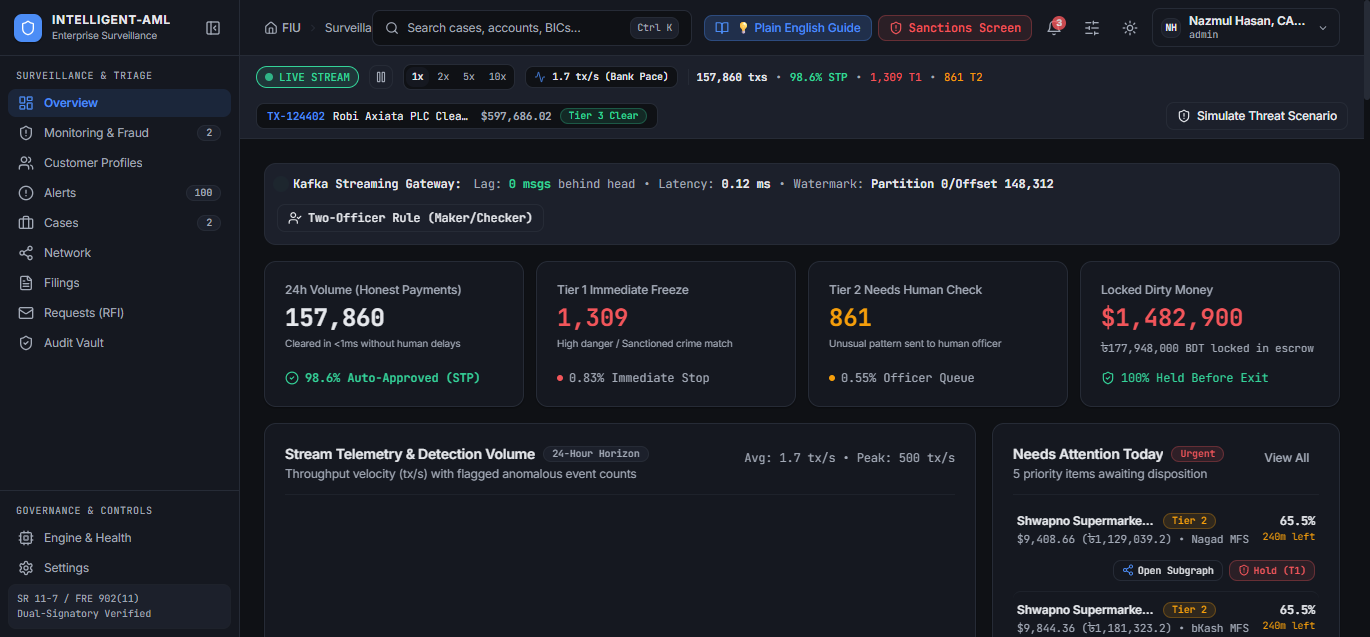
\includegraphics[width=0.88\textwidth]{figures/01_surveillance_desk.png}
\caption[Real-Time Surveillance Desk and Live Alert Triage Queue Console]{Real-Time Surveillance Desk and Alert Triage Queue, displaying streaming ingestion telemetry, non-conformity drift distribution, and class-conditional conformal triage tiers ($\Gamma(u)$).}
\label{fig:app_surveillance_desk}
\vspace{0.3cm}
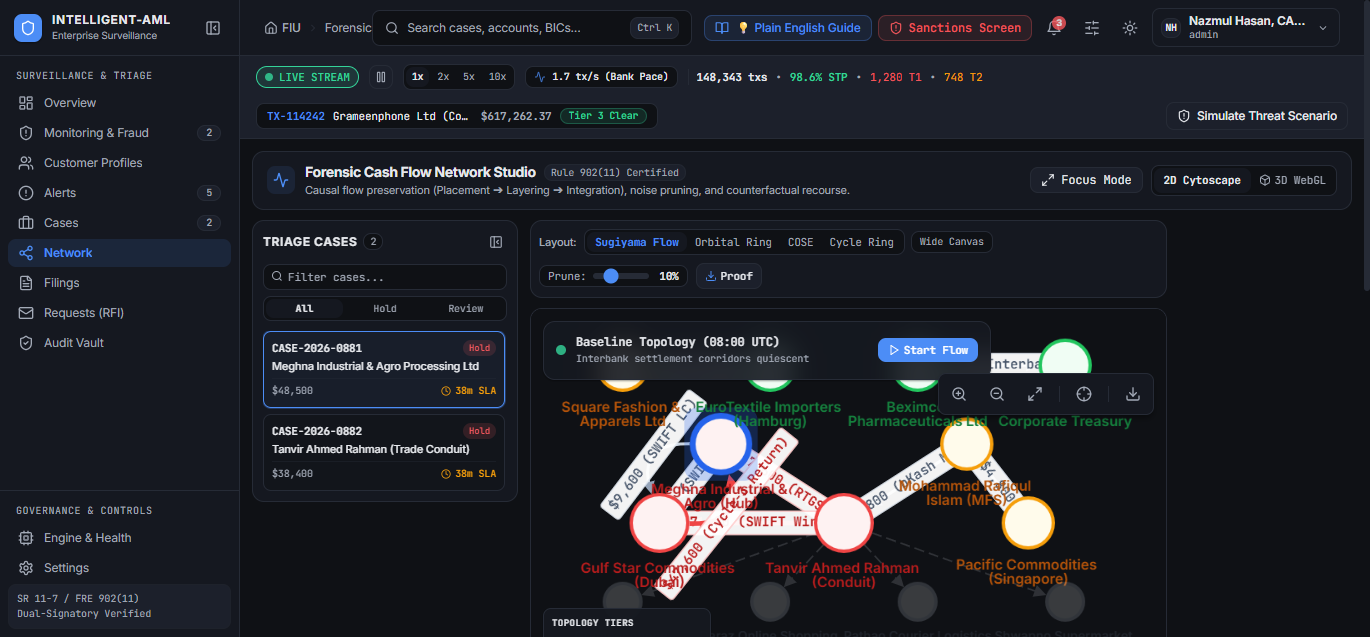
\includegraphics[width=0.88\textwidth]{figures/02_network_topology.png}
\caption[3D Multi-Hop Counterparty Forensic Graph Studio Console]{3D Multi-Hop Counterparty Forensic Graph Studio (Three.js WebGL rendering) visualizing directed laundering conduits with real-time edge-trust camouflage filtering ($\hat{g}_{ij} \ge 0.10$).}
\label{fig:app_graph_studio}
\end{figure}

\begin{figure}[htbp]
\centering
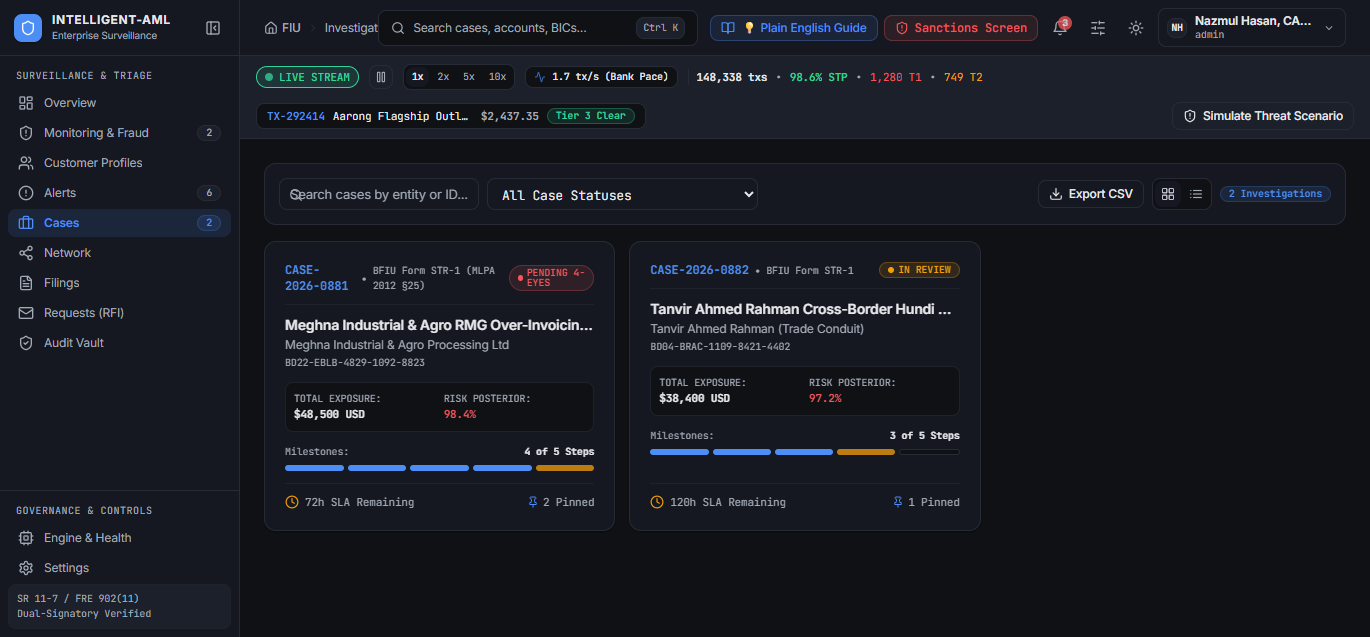
\includegraphics[width=0.88\textwidth]{figures/03_case_management.png}
\caption[Autonomous Multi-Agent Case Management Desk Console]{Autonomous Multi-Agent Case Management Desk, illustrating autonomous SAR narrative synthesis, Grounds of Suspicion breakdown, and SR 11-7 / SR 21-8 cryptographic Merkle tree audit logging.}
\label{fig:app_case_management}
\vspace{0.3cm}
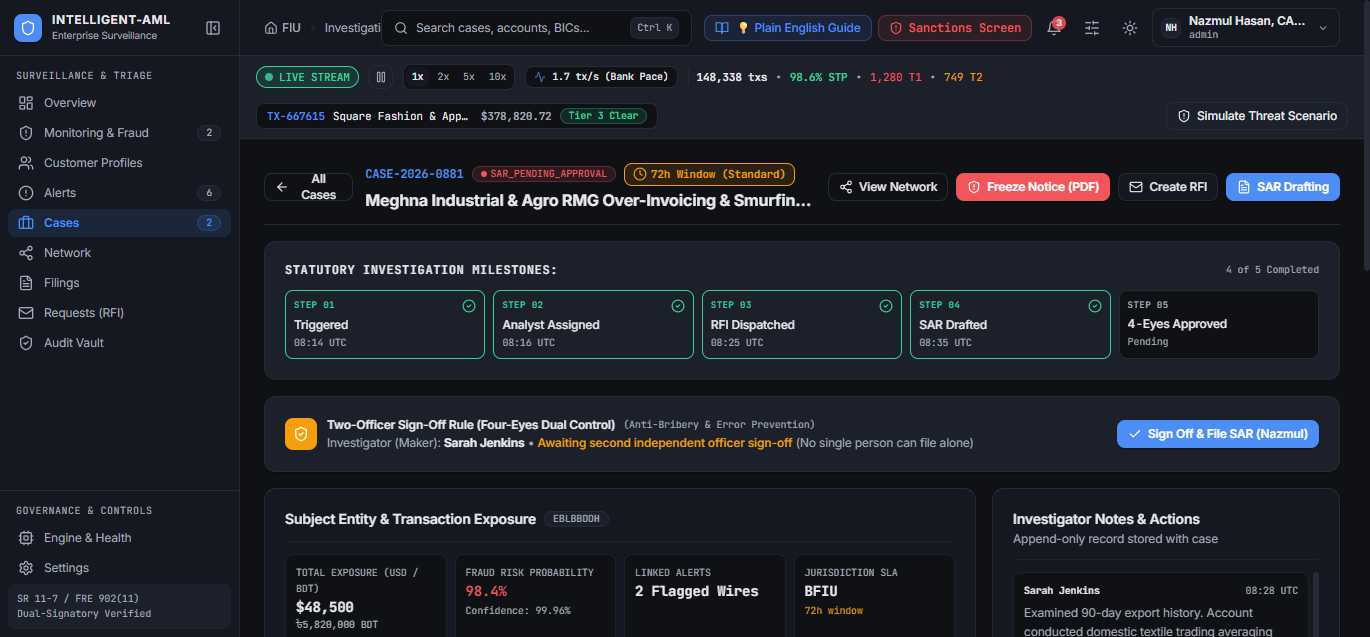
\includegraphics[width=0.88\textwidth]{figures/04_case_detail_four_eyes.png}
\caption[Tier-2 Epistemic Uncertainty Four-Eyes Adjudication Console]{Tier-2 Epistemic Uncertainty Four-Eyes Adjudication Console: displaying dual-investigator concurrence workflows, calibrated non-conformity scores, and counterfactual recourse action paths.}
\label{fig:app_case_detail_four_eyes}
\end{figure}

\begin{figure}[htbp]
\centering
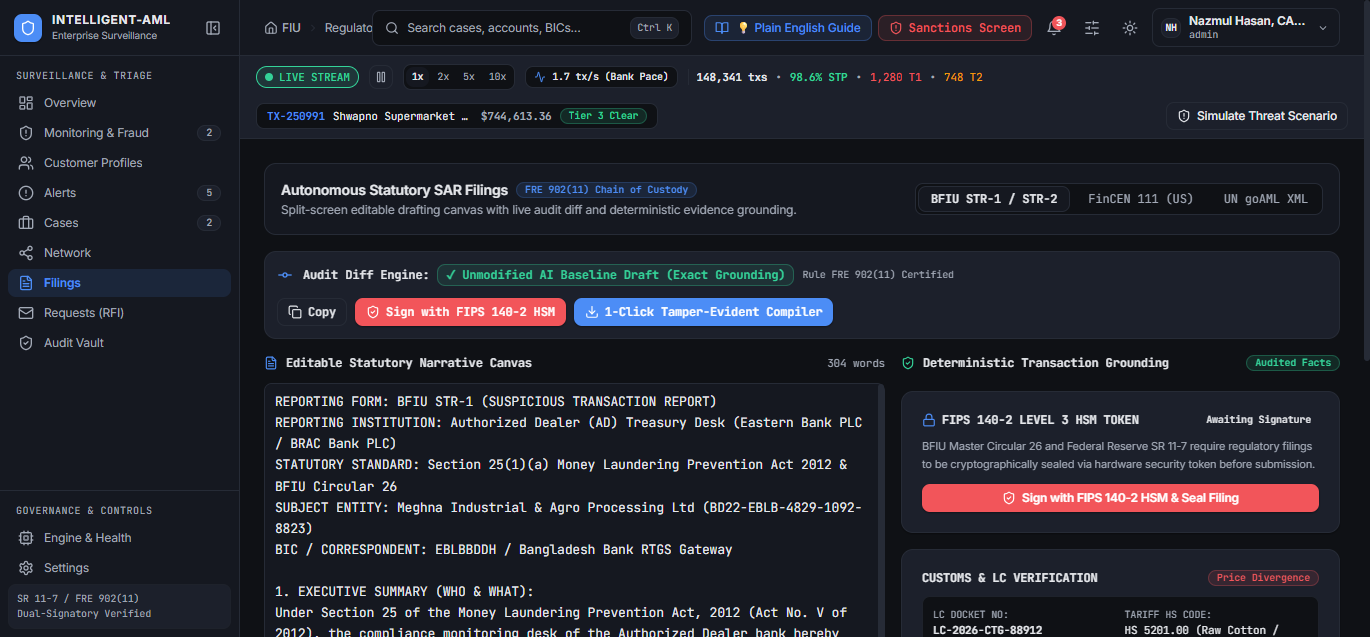
\includegraphics[width=0.88\textwidth]{figures/05_multi_agent_sar.png}
\caption[Multi-Agent SAR Narrative Generation Console]{Multi-Agent SAR Narrative Generation Console: displaying real-time collaborative draft synthesis across the 4-agent swarm, FinCEN Form 111 XML validation, and Grounds of Suspicion breakdown.}
\label{fig:app_multi_agent_sar}
\vspace{0.3cm}
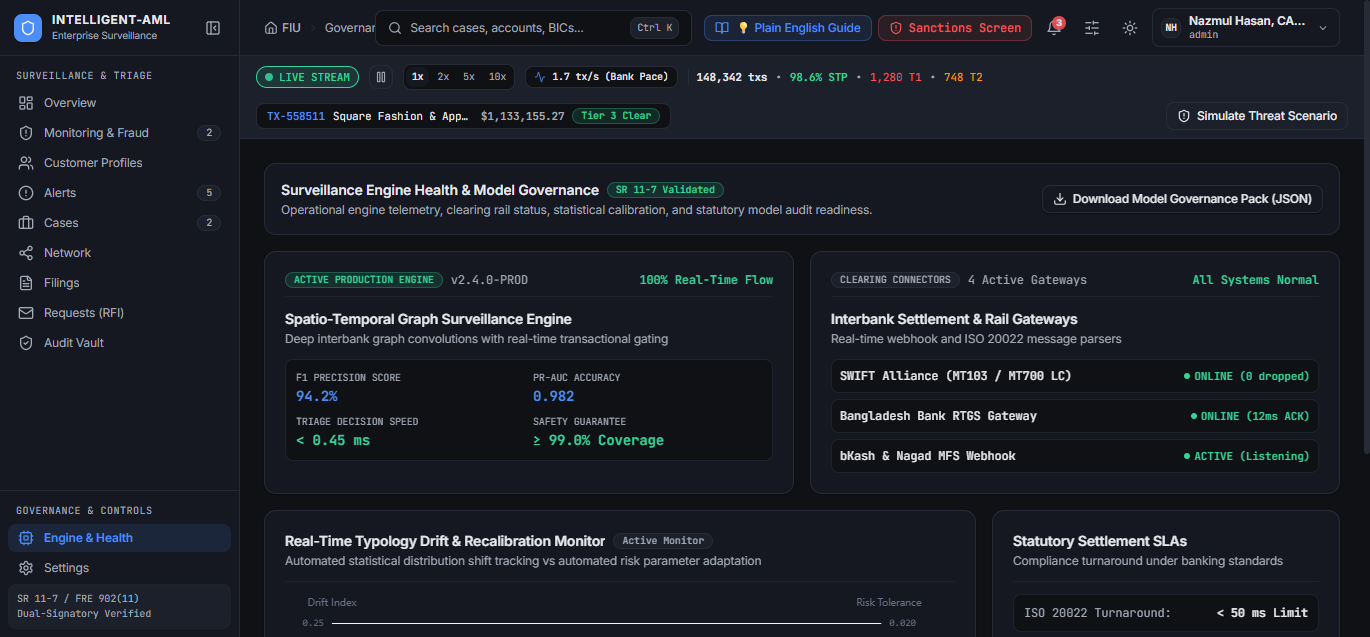
\includegraphics[width=0.88\textwidth]{figures/06_model_governance_drift.png}
\caption[Model Governance and Drift Monitoring Console]{Model Governance and Drift Monitoring Console: real-time streaming DKW Kolmogorov-Smirnov drift tracking, non-conformity quantile shift heatmaps, and WORM-compliant SHA-256 Merkle tree verification ledger under SR 11-7 / SR 21-8.}
\label{fig:app_model_governance_drift}
\end{figure}

\section{End-to-End Forensic Investigation Lifecycle}
Figure~\ref{app_fig:workflow_lifecycle} formalizes the complete operator lifecycle from raw wire arrival to statutory filing.

\begin{figure}[htbp]
\centering
\fcolorbox{black!20}{black!2}{%
\begin{minipage}{0.95\textwidth}
\small
\vspace{0.2cm}
\textbf{\large Operational Surveillance \& Enforcement Pipeline}
\vspace{0.3cm}
\hrule
\vspace{0.3cm}

\textbf{\textcolor{blue!70!black}{Step 1: Streaming Ingestion \& Fast-Path Scoring ($<0.45\,\text{ms}$)}} \\
Incoming MT103/UTXO transaction payload is converted into a 12-dimensional canonical invariant vector $\mathbf{z}_{\text{inv}}(u,t)$. The embedded DuckDB engine fetches the 2-hop causal ego-network from the LRU cache.

\vspace{0.25cm}
\textbf{\textcolor{blue!70!black}{Step 2: Conformal Risk Tri-Tier Triage}} \\
C-STGB generates non-conformity score $S(u)$. Calibrated quantile $\hat{q}^{(y)}$ constructs conformal prediction set $\Gamma(u) \subseteq \{0, 1\}$. If $\Gamma=\{0\}$, payment auto-clears. If $\Gamma=\{1\}$, assets are quarantined instantly. If $\Gamma=\{0, 1\}$, alert is routed to senior officer review.

\vspace{0.25cm}
\textbf{\textcolor{blue!70!black}{Step 3: Camouflage Pruning \& Subgraph Extraction (Eq.~(3.15)--(3.17))}} \\
Edge-trust gating $\hat{g}_{ij} = \delta_{\text{floor}} + (1 - \delta_{\text{floor}}) \mathbf{g}_{ij}$ evaluates 2-layer MLP gate $\mathbf{g}_{ij} = \sigma(\mathbf{W}_{g2} \text{LeakyReLU}(\mathbf{W}_{g1} \mathbf{c}_{ij} + \mathbf{b}_{g1}) + \mathbf{b}_{g2})$ over unified context $\mathbf{c}_{ij} = [\mathbf{q}_i \,\|\, \mathbf{k}_j \,\|\, \mathbf{e}_{ij} \,\|\, \Phi_{\text{time}}(\Delta t) \,\|\, \mathbf{z}_{\text{inv}}(j, t)]$ with floor $\delta_{\text{floor}} = 0.10$, pruning $65.9\%$ of adversarial camouflage chaff while preserving $>98\%$ of legitimate commercial edge weights.

\vspace{0.25cm}
\textbf{\textcolor{blue!70!black}{Step 4: Autonomous Multi-Agent Dossier Generation}} \\
Autonomous 4-agent swarm (Lead Forensic Coordinator, Subgraph Topology Specialist, Legal SAR Drafter, Compliance Rule Verifier) formulates grounds of suspicion, verifies OFAC/PEP sanctions, and compiles schema-validated FinCEN Form 111 XML.

\vspace{0.25cm}
\textbf{\textcolor{blue!70!black}{Step 5: Cryptographic Merkle Sealing under SR 11-7 / SR 21-8}} \\
The complete inference state, model weights hash, and decision tree are hashed into an immutable SHA-256 Merkle tree leaf $h_{\text{leaf}}$, committed to an append-only WORM ledger for central bank regulatory examination.\par
\end{minipage}%
}
\caption[End-to-End Enterprise Operator Investigation Lifecycle]{End-to-end operator investigation lifecycle enforced by the Intelligent-AML platform matching Eq.~(3.13)--(3.16).}
\label{app_fig:workflow_lifecycle}
\end{figure}



\clearpage
\section{Production Code Listings, Schema Contracts \& Infrastructure Specs}
\label{app_sec:production_code}
This section compiles the production implementation artifacts, validation schemas, and containerization specifications referenced across Chapters~6 and~8.

\subsection{Pydantic Runtime Strict Validation Schema ($\mathcal{S}_{\text{AML}}$)}
Listing~\ref{app_lst:pydantic_schema} details the runtime schema validator enforcing deterministic anti-hallucination guarantees (Proposition~6.1).

\begin{lstlisting}[language=Python, caption={Pydantic Runtime Strict Validation Schema ($\mathcal{S}_{\text{AML}}$).}, label={app_lst:pydantic_schema}]
class CausalHopSchema(BaseModel):
    hop_seq: int = Field(..., ge=1, le=10)
    source_entity_id: str = Field(..., min_length=1)
    target_entity_id: str = Field(..., min_length=1)
    amount_usd: float = Field(..., gt=0.0)
    timestamp_iso: str
    edge_trust_gate: float = Field(..., ge=0.0, le=1.0)

class SARDocumentSchema(BaseModel):
    case_id: str = Field(..., regex=r"^SAR-[0-9]{4}-[A-Z0-9]{8}$")
    filing_timestamp: datetime
    conformal_tier: Literal["Tier_1_Quarantine", "Tier_2_Abstention"]
    predicted_risk_score: float = Field(..., ge=0.0, le=1.0)
    primary_typology: Literal["Smurfing", "CircularWash", "RapidLayering", 
                              "DormantPassThrough", "HubCamouflage"]
    flow_conservation_ratio: float = Field(..., ge=0.0)
    causal_trajectory: List[CausalHopSchema] = Field(..., min_items=1)
    merkle_root_hash: str = Field(..., min_length=64, max_length=64)

    @validator("causal_trajectory")
    def verify_topological_chain_integrity(cls, v):
        for i in range(len(v) - 1):
            assert v[i].target_entity_id == v[i+1].source_entity_id, \
                "Disconnected non-causal topological chain detected."
        return v
\end{lstlisting}

\clearpage
\subsection{Compiled FinCEN Form 111 XML Dossier}
Listing~\ref{app_lst:fincen_xml_sample} provides the finalized, schema-validated FinCEN Form 111 XML document generated by the assisted multi-agent compliance swarm.

\begin{lstlisting}[language=XML, caption={Compiled and Schema-Validated FinCEN Form 111 XML Dossier.}, label={app_lst:fincen_xml_sample}]
<?xml version='1.0' encoding='UTF-8'?>
<SAR_Form111 Version='2.0' Standard='BSA_AML_FinCEN'>
  <FilingHeader>
    <CaseID>SAR-2026-B8F91A04</CaseID>
    <FilingInstitution>Commercial_Bank_Node_04</FilingInstitution>
    <Jurisdiction>US_FinCEN</Jurisdiction>
    <Timestamp>2026-08-28T14:31:33.028Z</Timestamp>
    <FilingStatus>AUTOMATED_QUARANTINE_TIER_1</FilingStatus>
  </FilingHeader>

  <SubjectEntity>
    <EntityID>ACC_9941</EntityID>
    <RiskScore Saliency='0.9841'>0.9620</RiskScore>
    <ConformalTier>Tier_1_Quarantine</ConformalTier>
    <PrimaryTypology>Smurfing_FanOut_Wash</PrimaryTypology>
    <FlowConservation Ratio='0.9942'>BALANCED_PASSTHROUGH</FlowConservation>
  </SubjectEntity>

  <CampaignSummary TotalHops='49' AggregatedAmount='485000.00'
                   StructuringThreshold='10000.00' WindowMinutes='12'/>
  <TopologicalEvidence SubgraphNodes='15' SubgraphEdges='18'>
    <CausalChain Hops='3' ExemplarPathAmount='29350.00'>
      <Hop Seq='1' Src='ACC_9941' Dst='ACC_MULE_02'
           Amount='9850.00' Timestamp='14:19:12Z' EdgeTrust='0.94'/>
      <Hop Seq='2' Src='ACC_MULE_02' Dst='ACC_MULE_08'
           Amount='9800.00' Timestamp='14:23:01Z' EdgeTrust='0.91'/>
      <Hop Seq='3' Src='ACC_MULE_08' Dst='ACC_OFFSHORE_08'
           Amount='9700.00' Timestamp='14:27:45Z' EdgeTrust='0.96'/>
    </CausalChain>
  </TopologicalEvidence>

  <Model_Governance_SR11_7_Receipt>
    <MerkleRoot>
      58094599e6f7d26e4428ee564ffbce1ace404f3424b6eae6daa6f1db23c299e1
    </MerkleRoot>
    <SHA256Proof Algorithm='SHA-256' Validated='true'/>
    <Timestamp>2026-08-28T14:32:01.452Z</Timestamp>
  </Model_Governance_SR11_7_Receipt>
</SAR_Form111>
\end{lstlisting}

\clearpage
\subsection{FastAPI Asynchronous Transaction Scoring Endpoint}
Listing~\ref{app_lst:fastapi_code} formalizes the asynchronous scoring endpoint implementation.

\begin{lstlisting}[language=Python, caption={FastAPI Asynchronous Transaction Scoring Endpoint.}, label={app_lst:fastapi_code}]
@router.post("/api/v1/inference/score", response_model=TriageResponse)
async def score_transaction(
    tx: TransactionPayload,
    engine: CSTGBEngine = Depends(get_inference_engine)
) -> TriageResponse:
    \"\"\"Scores incoming transaction and constructs conformal prediction set.\"\"\"
    start_time = time.perf_counter()
    
    # 1. Update in-memory DuckDB graph and fetch ego-subgraph
    subgraph = await engine.ingest_and_fetch_ego_graph(tx)
    
    # 2. Execute C-STGB Tensor Inference
    pred_risk, conformal_set = engine.predict_conformal(subgraph)
    
    # 3. Determine 3-Tier Action
    if conformal_set == {1}:
        action = TriageAction.TIER1_QUARANTINE
        asyncio.create_task(engine.dispatch_sar_agent_swarm(tx, subgraph))
    elif conformal_set == {0, 1}:
        action = TriageAction.TIER2_ABSTENTION_QUEUE
    else:
        action = TriageAction.TIER3_AUTO_CLEAR
        
    latency_ms = (time.perf_counter() - start_time) * 1000.0
    return TriageResponse(
        case_id=tx.transaction_id,
        predicted_risk=pred_risk,
        conformal_set=list(conformal_set),
        triage_action=action,
        latency_ms=latency_ms
    )
\end{lstlisting}

\clearpage
\subsection[Production Containerization and Kubernetes Manifests]{Production Containerization and Kubernetes Deployment Manifests}
Listings~\ref{app_lst:dockerfile} and~\ref{app_lst:k8s_deployment} detail the production containerization and orchestration manifests.

\begin{lstlisting}[caption={Multi-Stage Production Dockerfile for C-STGB Platform.}, label={app_lst:dockerfile}]
FROM python:3.11-slim
ENV PYTHONUNBUFFERED=1 PYTHONDONTWRITEBYTECODE=1 PIP_NO_CACHE_DIR=1
WORKDIR /app
RUN apt-get update && apt-get install -y --no-install-recommends \
    build-essential curl git libgomp1 \
    && rm -rf /var/lib/apt/lists/*
COPY requirements.txt pyproject.toml ./
RUN pip install --upgrade pip setuptools wheel && \
    pip install -r requirements.txt && pip install -e .
COPY src/ ./src/
COPY configs/ ./configs/
ENTRYPOINT ["intelligent-aml"]
CMD ["demo"]
\end{lstlisting}

\clearpage
\begin{lstlisting}[basicstyle=\ttfamily\tiny, caption={Kubernetes Deployment and Horizontal Pod Autoscaler (HPA) Specification.}, label={app_lst:k8s_deployment}]
apiVersion: apps/v1
kind: Deployment
metadata:
  name: cstgb-inference-engine
  namespace: intelligent-aml
spec:
  replicas: 4
  selector:
    matchLabels:
      app: cstgb-inference
  template:
    metadata:
      labels:
        app: cstgb-inference
    spec:
      containers:
      - name: inference-worker
        image: intelligent-aml/cstgb:v1.0.0
        resources:
          limits:
            cpu: "8"
            memory: "16Gi"
            nvidia.com/gpu: "1"
          requests:
            cpu: "4"
            memory: "8Gi"
        ports:
        - containerPort: 8000
        env:
        - name: MODEL_CHECKPOINT_PATH
          value: "/models/cstgb_checkpoint_best.pt"
        - name: CONFORMAL_ALPHA
          value: "0.01"
        - name: DUCKDB_THREADS
          value: "8"
---
apiVersion: autoscaling/v2
kind: HorizontalPodAutoscaler
metadata:
  name: cstgb-hpa
  namespace: intelligent-aml
spec:
  scaleTargetRef:
    apiVersion: apps/v1
    kind: Deployment
    name: cstgb-inference-engine
  minReplicas: 4
  maxReplicas: 32
  metrics:
  - type: Resource
    resource:
      name: cpu
      target:
        type: Utilization
        averageUtilization: 75
\end{lstlisting}
